\documentclass[3p,twocolumn]{elsarticle}
%\documentclass[review]{elsartical}%sigal column



\journal{Journal of \LaTeX\ Templates}

\bibliographystyle{elsarticle-num}
%%%%%%%%%%%%%%%%%%%%%%%

\usepackage{amsmath,amssymb}

\usepackage{picins}
\usepackage{picinpar}
\usepackage{algorithm}
\usepackage{algorithmic}

\usepackage{lineno,hyperref}
\modulolinenumbers[5]

\begin{document}

\begin{frontmatter}

\title{A survey: Sparse Representation in Geometry Processing\tnoteref{mytitlenote}}
%\tnotetext[mytitlenote]{Fully documented templates are available in the elsarticle package on \href{http://www.ctan.org/tex-archive/macros/latex/contrib/elsarticle}{CTAN}.}
%
%%% Group authors per affiliation:
%\author{Elsevier\fnref{myfootnote}}
%\address{Radarweg 29, Amsterdam}
%\fntext[myfootnote]{Since 1880.}
%
%%% or include affiliations in footnotes:
%\author[mymainaddress,mysecondaryaddress]{Elsevier Inc}
%\ead[url]{www.elsevier.com}
%
%\author[mysecondaryaddress]{Global Customer Service\corref{mycorrespondingauthor}}
%\cortext[mycorrespondingauthor]{Corresponding author}
%\ead{support@elsevier.com}
%
%\address[mymainaddress]{1600 John F Kennedy Boulevard, Philadelphia}
%\address[mysecondaryaddress]{360 Park Avenue South, New York}

\begin{abstract}
\end{abstract}

\begin{keyword}
\texttt{elsarticle.cls}\sep \LaTeX\sep Elsevier \sep template
\MSC[2010] 00-01\sep  99-00
\end{keyword}

\end{frontmatter}

\linenumbers

%\begin{itemize}
%\item document style
%\end{itemize}
%
%\begin{enumerate}[(1)]
%\item Group the authors per affiliation.
%\item Use footnotes to indicate the affiliations.
%\end{enumerate}

\section{Introduction}
\label{sec:introduction}

Because of the fast development of Internet and other electronic equipments, the size of dataset is becoming  incredibly massive.
How to extract compact knowledge from such massive datasets is yet to be resolved.
At the same time, the dimension of data becomes much higher than before.
Thus how to extract low-dimensional structures from high-dimensional data is another serious problem in modern signal processing.

To solve these two challenging problems, sparsity-based approaches have been successfully introduced in many applications.
Sparse representation which models data vectors as sparse linear combinations of basis elements, is widely used in machine learning, signal processing, neuroscience and statistics.
Dictionary learning learns an overcomplete dictionary which owns the ability to represent given signals.
Low rank representation which decomposes a given matrix into a low rank matrix and residual with certain property.
So far sparse techniques have become state-of-art tools in many fields like machine learning, data mining, computer vision, pattern recognition etc.
%Sparse representation of signals has been drawing much attention of the researchers.

In geometric processing and computer graphics, people start to find out the advantages of sparse techniques.
Better results are obtained with sparse techniques.
At the same time, most formulations cannot be directly applied on geometric problems.
Thus many non-trivial problems must be solved while applying sparse techniques.
We would like to show how sparse technique, a strong tool in machine learning is brought into a fresh filed, geometric processing.

In the rest of this paper, we first introduce traditional sparse models used in machine learning and computer vision.
Then we illustrate how people in geometric processing use sparse techniques in different applications.

\input{Pre}
\input{Sparse}
\section{Sparse Representation in Geometry Processing}
\label{sec:L0}

In this section we will give the survey of sparse representation in geometry processing according to its continuous promotion.

\subsection{$l_0$-norm}

At the very beginning of the development of sparse representation, the $l_0$ norm of a vector counts the number of non-zero entries, which directly measures sparsity, here we call it standard sparse representation. Mathematically, a signal $x\in R^{N}$ can be represented as a linear combination of a few atoms from a overcomplete dictionary $\mathbf{D}_{n \times m}$, i.e., $x\approx\mathbf{D}\alpha$, via $l_0$-minimization:
\begin{equation}
 \label{eq:L0 modeling}
 \alpha_{x} = \arg\min_{\alpha}||\alpha||_0, s.t. ||x-\mathbf{D}\alpha||_2 \le \varepsilon
\end{equation}
where, as mentioned above, $\|\centerdot\|_0$ counts the number of the non-zero coefficients in $\alpha$, and $\varepsilon$ is a small constant balancing the sparsity and the approximation error. Matching Pursuit(MP)\cite{mallat1993matching} and its variant Orthogonal Matching Pursuit(OMP)\cite{pati1993orthogonal} is well known in generating the solution which is out of the scope of this article.

Since this norm is difficult to optimize directly due to its combinational nature requiring that one enumerate all possible $k$-element collections of $\mathbf{D}$, for $k=1,2,...,m$, such an algorithm would cost at least $O(2^{m})$ flops to carry out in general, and at least $O(m^{k})$ even when a sparse $k$-element represent existed, there are not many works based on it.

\paragraph{Modeling}Modeling with constraints is an important tool for the construction and modification of 3D geometric models. Especially in the case of modeling man-made structure like architecture or machine parts, geometric constraints are able to create and preserve ubiquitous alignment properties like element parallelism, conllinearity, fixed angles and distances, or symmetry relations. Existing approaches to analyze and solve constraint systems usually fail to meet two main challenges of an interactive 3D modeling system: for each atomic editing operation, it is crucial to adjust as few auxiliary vertices as possible in order to not destroy the user's earlier editing effort; the whole constraint resolution pipeline is required to run in real-time to enable a fluent, interactive workflow.

To address both issues, \cite{habbecke2012linear} presents a novel interactive constrained modeling with a well-defined strategy that, for an atomic editing operation, computes as small as possible model updates in terms of the total number of adjusted vertices. Briefly, a model instance $\mathbf{X}_0$, whose elements are the vertex positions, satisfies all constraints denoted by $\mathbf{c(X_0)=0}$ which is a vector-valued function. Then for a given editing displacement $\mathbf{d}$, the central goal is to find a correction displacement $\mathbf{d'}$ such that $\mathbf{c(X_0+d+d')=0}$, where the zero elements of $\mathbf{d'}$ and $\mathbf{d}$ are disjoint and $\mathbf{d'}$ should be as sparse as possible. Figure... shows the result.

\begin{figure}[ht]
  \centering
  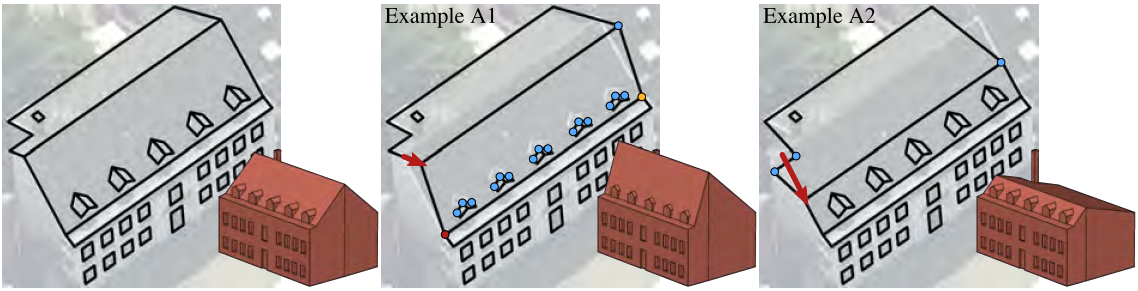
\includegraphics[width=3in]{images/modeling_L0}
  \caption{$l_0$ optimization: constrained modeling\cite{habbecke2012linear}. Left: original configuration. Center: editing operation such that the base plane of the dormers changes its orientation(example A1). Right: the dormers' base plane does not change(example A2). Blue vertices are relaxed in the analysis phase and automatically updated by the editing system.}
\end{figure}

\paragraph{Mesh denoising} Mesh denoising is an important tool in geometry processing. A wide variety of denoising algorithms already exist that can be divided into two approaches: prescribed differential information based and extending the bilateral filter from 2D signal processing to arbitrary 3D meshes. But it is inherently challenging as it can be difficult to distinguish features from noise.

Last year, \cite{he2013mesh} extends the image $l_0$-smoothing method\cite{xu2011image} to denoise triangulated meshes of 3D models with a new developed discrete gradient operator on arbitrary triangle meshes. The goal is to minimize the curvature of the surface except at sharp features instead of creating piecewise constant functions as was done for images. Due to the nature of $l_0$ norm, this work can handle large amount of noise and produce high quality results except some shapes with extreme triangulations that the only vertices that exist lie at sharp features in the model. Figure... shows the results.

\begin{figure}[ht]
  \centering
  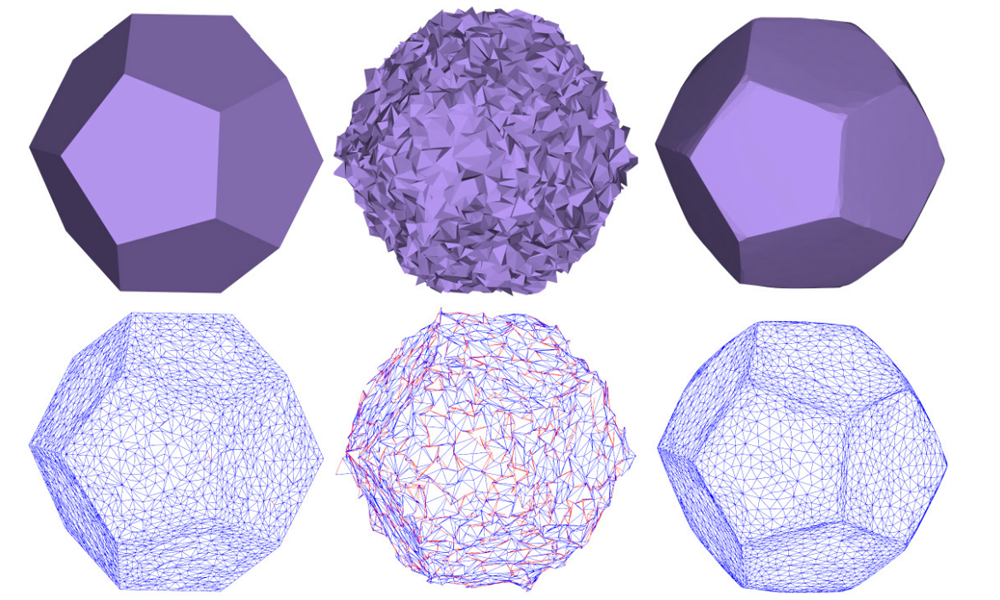
\includegraphics[width=3in]{images/denoise_L0}
  \caption{$l_1$ optimization: mesh denoising\cite{he2013mesh}. Left: initial surface. Center: surface corrupted by Gaussian noise in random directions with standard deviation $\sigma=0.4l_{e}$($l_{e}$ is the mean edge length). Right: denoising result. The wireframe shows folded triangles as red edges.}
\end{figure}

To apply sparse representation in images and graphics better, several promotions of $l_0$ norm have been proposed based on which there are much more works in recent years.

\label{sec:L1}

\subsection{$l_1$ norm}

A more formal approach convexifies $(1)$ by replacing the $l_0$ norm with an $l_1$ norm:
\begin{equation}
 \label{eq:L1 modeling}
 \alpha_{x} = \arg\min_{\alpha}||\alpha||_1, s.t. ||x-\mathbf{D}\alpha||_2 \le \varepsilon
\end{equation}
This can be cast as a linear Programming(LP) problem, for which solutions are available even in large-scale problems, owing to modern interior-point linear programming methods. This approach to overcomplete signal representation was called Basis-Pursuit(BP)\cite{chen1998atomic}, which observed that it sometimes gave highly sparse solutions to problems known to have such solutions, and showed that it could, in specific cases, outperform the greedy Matching Pursuit approach in generating sparse solutions.

Considering these advantages, $l_1$ norm comprises a large proportion of sparse representation in geometry processing.

\paragraph{Reconstruction}In recent years, many robust surface reconstruction techniques have been developed that can deal with a variety of acquisition errors like noise, outliers, missing data(holes) or registration artifacts. They are commonly based on a robust $l_1$ optimization approach and are able to produce high-quality output despite very difficult data.

Actually, the idea of $l_1$ optimization has a long history. Decades ago, \cite{weber1909theory} had proposed the optimal location problem which is a statistical tool that is traditionally applied globally to multivariate non-parametric point-samples to generate a good representative for a large number of samples in the presence of noise and outliers. This problem is known as $l_1$ median\cite{brown1983statistical,small1990survey} in statistic finding a robust global center of an arbitrary set of points.

\cite{lipman2007parameterization} applies this tool locally in a geometric context and introduces a parameterization-free local projection operator(LOP) which does not rely on estimating a local normal. LOP robustly fits a set of resampling points to a noisy point cloud((a) in Figure...) by iteratively applying a system attractive forces defined by the input points and is particulary attractive for reconstruction since it does not put many constraints on the nature of the input data, i.e., it does not require a well-defined surface parameterization nor a surface which can be locally well approximated with a plane. But LOP is subject to a local density parameter, i.e., the result is affected by the points distributions.

Considering the limitation of LOP for non-uniform distributions common in raw data, a weighted LOP(WLOP) by modifying and extending LOP operator in \cite{huang2009consolidation} which is a two phase method focusing on reliable normal estimation to consolidate an unorganized point cloud is proposed. Actually, it is just a preprocess of the input point cloud((b) in Figure...). By taking into account a local density measure, WLOP is first used to produce a set of denoised, outlier-free and evenly distributed points to improve the reliability of local PCA for initialization of normals which are used in the following normal estimation phase. But it lacks of theoretic guarantee and cannot address the missing data problem like LOP.

In fact, LOP requires high computational effort due to the nature of $l_1$ optimization. To improve efficiency, \cite{preiner2014CPF} presents a novel continuous formulation of the WLOP operator based on a Gaussian mixture describing the input point density to make a robust reconstruction at interactive frame rates for moderately sized dynamic point sets possible((c) in Figure...).

In addition to these $l_1$ median based works mentioned above, \cite{avron2010L1} introduces an $l_1$ sparse method decoupling orientations and positions for the reconstruction of a piecewise smooth point set surface with sharp feature((d) in Figure...). They first solve for the point orientations and then, based on the piecewise smooth normals, solve for the point positions. Both problems are formulated in a similar $l_1$ nature, yielding a consistent solution.

Figure...shows all the reconstruction results of these methods.

\begin{figure}[ht]
  \centering
  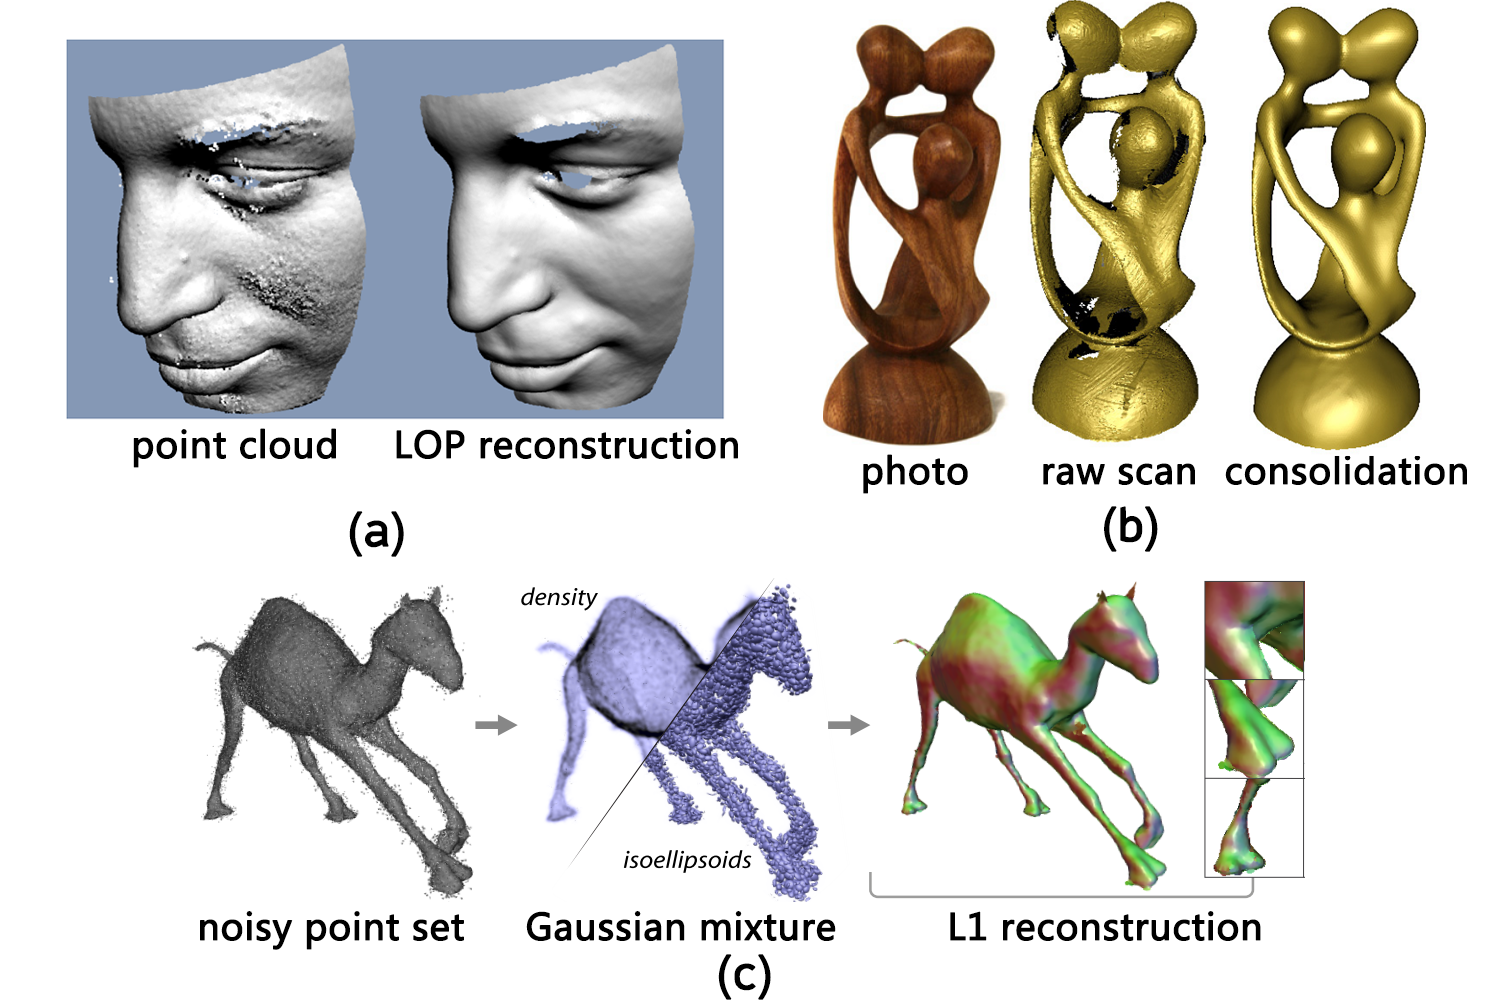
\includegraphics[width=3in]{images/reconstruction_L1}
  \caption{$l_1$ optimization: reconstruction results. (a): \cite{lipman2007parameterization}. (b): \cite{huang2009consolidation}. (c): \cite{preiner2014CPF}. (d): \cite{avron2010L1}.}
\end{figure}

\paragraph{Skeleton extraction}Skeletal shape representations have been intensely studied in various fields and utilized in a variety of applications for shape modeling and analysis. \cite{huang2013l1} finds out a new application for $l_1$ median, they introduce $l_1$-medial skeleton as a curve skeleton representation for 3D point cloud data(Figure...). Without building any point connectivity or estimating point normals, they directly project point samples onto their local centers as $l_1$ medians with growing neighborhood and push the projected samples via conditional regularization to obtain a uniform distribution of samples along skeleton branches. It is a simple but powerful approach for extracting skeletons from unorganized, unoriented and incomplete 3D raw point clouds.

\begin{figure}[ht]
  \centering
  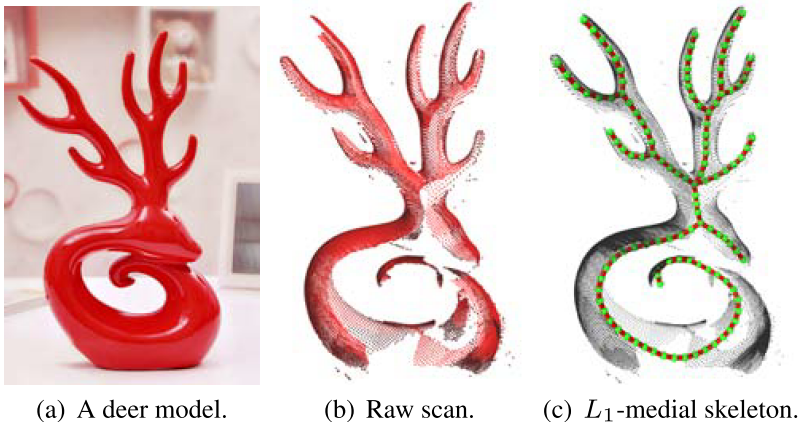
\includegraphics[width=3in]{images/skeleton_L1}
  \caption{$l_1$ optimization: skeleton extraction\cite{huang2013l1}. Given an unorganized, unoriented, and incomplete raw scan with noise and outliers, a complete and quality curve skeleton is extracted.}
\end{figure}

\paragraph{Mesh Denoising} Like \cite{he2013mesh} mentioned above, most previous methods rely on computation of differential properties to detect noise which is unreliable and unstable and require the user to carefully tune the model parameters case by case and rarely have theoretical guarantees. To address these problems, \cite{wang2014decoupling} presents a two phase approach for decoupling features and noise on discrete surfaces. After generating a base mesh which is obtained by denoising the input data using a global Laplacian regularization smoothing optimization in which the smoothness parameter is automatically chosen by adopting the generalized cross-validation scheme, sharp features are extracted from the residual between base mesh and input mesh based on an $l_1$ analysis compressed sensing optimization. It is achieved by the discovery that sharp features can be sparsely represented in some coherent dictionary which is constructed by the pseudo-inverse matrix of the Laplacian of the shape, Figure... gives the 1D illustration and the denoising results. It is the first time noise and features are analyzed and separated in such an elegant manner with guarantees by statistical theory.

\begin{figure}[ht]
  \centering
  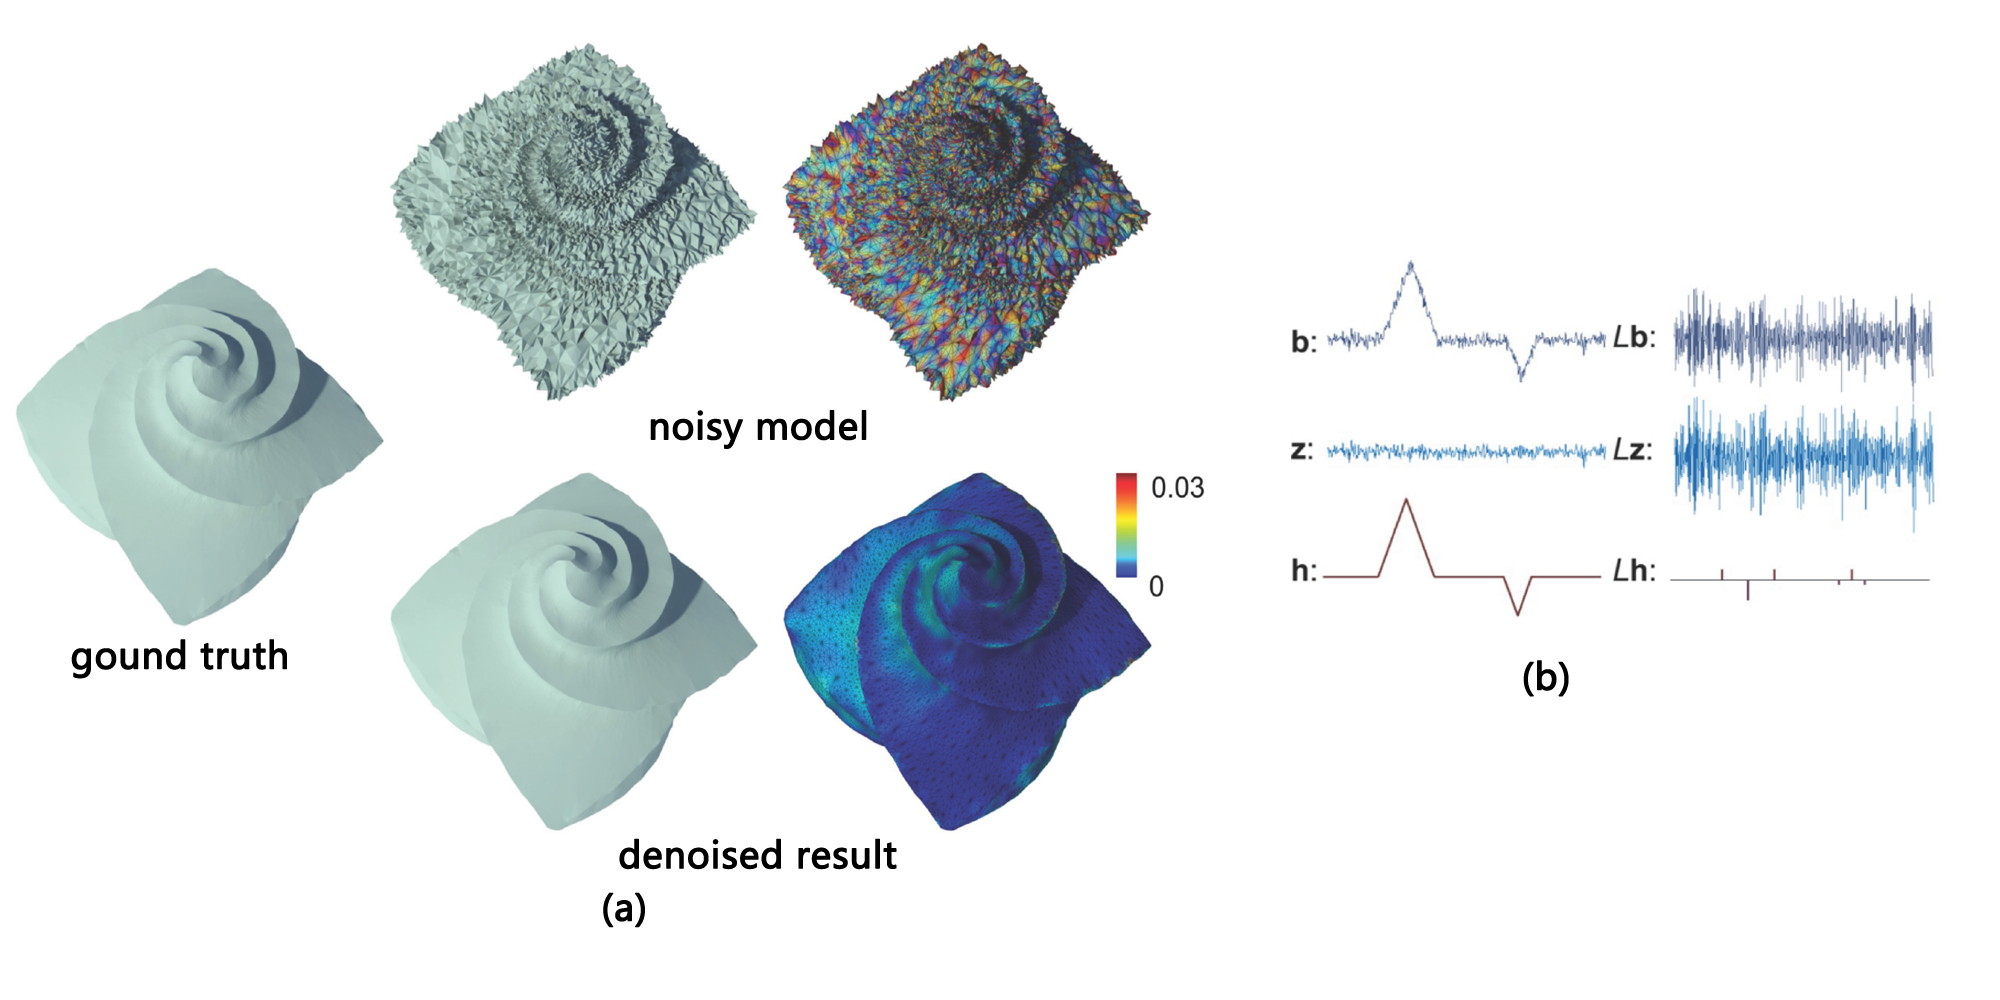
\includegraphics[width=3in]{images/denoise_L1}
  \caption{$l_1$ optimization: mesh denoising\cite{wang2014decoupling}. (a) is a denoising example. (b) is the 1D illustration of signals and their Laplacians. Left:the residual $\mathbf{b}$ (upper) is a mixture of noise $\mathbf{z}$(middle) and features $\mathbf{h}$(lower). Right: the corresponding Laplacians of signals on the left.}
\end{figure}

\paragraph{Shape Matching} Matching of deformable shapes is a notoriously difficult problem playing an important role in many application, non-rigid matching typically uses point-wise representation of correspondence, which results in the number of degrees of freedom growing exponentially with the number of matched points. \cite{pokrass2013sparse} poses the problem of finding intrinsic correspondence between near-isometric deformable shapes as a permuted sparse modeling. It is based on the observation that choosing the discretized eigenfunctions of the Laplace-Beltrami operator of two shapes will cause the low-distortion correspondence being represented by a nearly diagonal, and therefore very sparse matrix, and among other dense correspondence techniques, this method relies on the smallest amount of information. Figure...

\begin{figure}[ht]
  \centering
  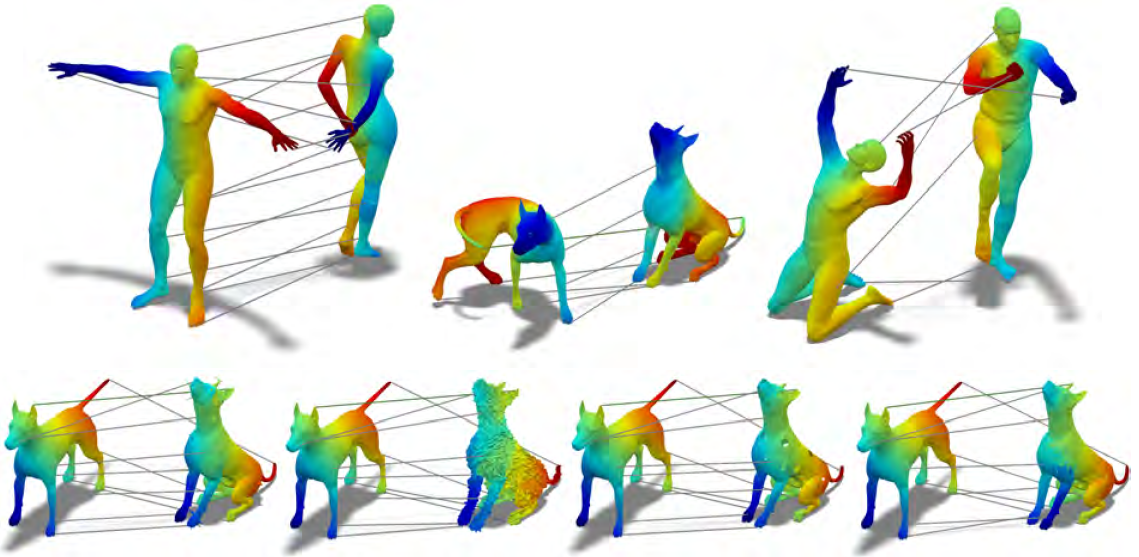
\includegraphics[width=3in]{images/matching_L1}
  \caption{$l_1$ optimization: shape matching\cite{wang2014decoupling}. First row: point-to-point correspondences between different non-isometric shapes. Second row: point-to-point correspondence between SHREC shapes undergoing nearly isometric deformations and noise.}
\end{figure}

\paragraph{Barycentric coordinates}

\begin{figure}[ht]
  \centering
  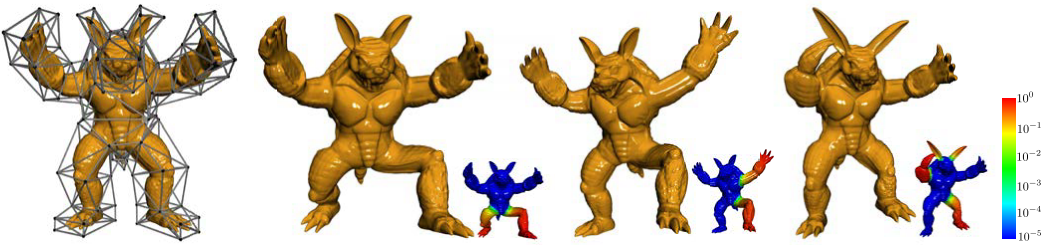
\includegraphics[width=3in]{images/LBC_L1}
  \caption{$l_1$ optimization: local barycentric coordinates\cite{}. Using LBC for 3D cage-based manipulation allows for local, smooth and shape-aware deformations. Only parts near the manipulated control points are deformed, as indicated by the color-coding.}
\end{figure}

In summary, many robust surface reconstruction techniques have been developed to deal with a variety of acquisition errors like noise, outliers, missing data(holes) or registration artifacts. They are commonly based on a robust $l_1$ optimization approach and are able to produce high-quality output despite very difficult data. Though typical $l_1$ norm problems aim at reconstructing sparse signals from a large amount of measurement. It has also been applied to some other problems like polycube, correspondence and denoising mentioned above. Most of the $l_1$ techniques are typically too expensive to achieve interactive reconstruction times for at least moderately sized point sets, even for parallel implementations. Even though they are designed for quality rather than performance due to their nature, the performance problem is worth researching. 
\label{sec:Lp}

\subsection{$l_{p}$ norm} Now we have overviewed the works based on $l_0$ and $l_1$ norm, how about the other values of $p$?

In fact, \cite{elad2010sparse} has given a brief discussion about it when $0<p<1$ and illustrate the tendency of $l_{p}$($0<p<1$) norm to drive results to become sparse. Then base on recent advances in sparsity-inducing penalties\cite{bach2012optimization,marjanovic2012optimization} that have been successfully applied in compressive sensing\cite{candes2008introduction}, \cite{bouaziz2013sparse} expresses the ICP registration problem as a sparse $l_{p}$ optmization$0\leq p\leq1$, obtain an heuristic-free, robust rigid registration algorithm. And \cite{chartrand2007exact} showing that $l_{p}$ norms with $p<1$ outperform the $l_1$ norm in inducing sparsity makes the optimization more resilient to a large number of outliers. Figure...is the registration results of sparse ICP under different values of $p$ among which it can be found that $0<p<1$ gives the best result, but how to automatically decide $p$ is not discussed.

\begin{figure}[ht]
  \centering
  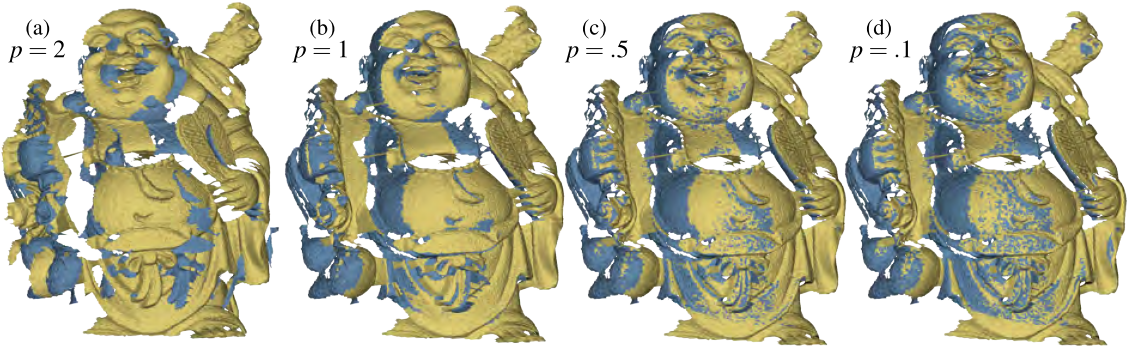
\includegraphics[width=3in]{images/sparseICP}
  \caption{$l_{p}$ optimization: registration using sparse ICP\cite{chartrand2007exact}.}
\end{figure}

In addition, there is still another kind of promotion for sparse representation. Sparse Subspace Clustering(SSC) \cite{elhamifar2009sparse} introduces compressed sensing techniques to subspace segmentation. SSC uses the sparsest representation produced by $l_1$ optimization to define the affinity matrix of an undirected graph. It is based on the observation that each point in a union of linear subspaces can always be represented as a linear combination of the points belonging to the same linear subspace. Inspired by SSC and \cite{cheng2011multi}, \cite{hu2012co} proposes a subspace clustering formulation of optimization with a consistent multi-feature penalty achieved with both $l_{2,1}$ norm and $l_{1,1}$ norm to guarantee the consistency of co-segmentation results according to various features. Briefly, after over-segmenting the input models into primitive patches(left in Figure...), they group the similar patches via a subspace clustering scheme. Figure...(right) is the co-segmentation result.

\begin{figure}[ht]
  \centering
  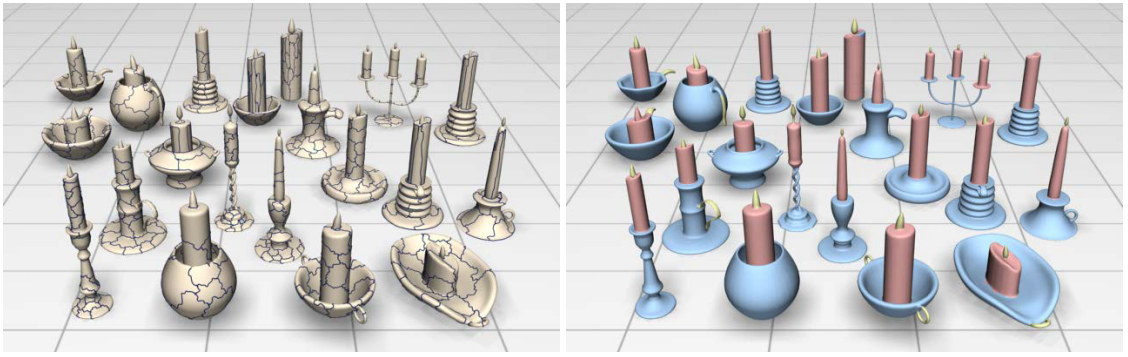
\includegraphics[width=3in]{images/co-segmentation}
  \caption{$l_{p}$ optimization: co-segmentation\cite{hu2012co}. Left: over segmented patches. Right: co-segmented result.}
\end{figure} 
\label{sec:Learning}

\subsection{Sparse Decomposition}

Sparse decomposition, just as the name implies, is a kind of matrix decomposition whose result matrices contain a simple matrix(e.g., transformation matrix\cite{le2012smooth}) and the correspondent coefficient matrix which is as sparse as possible. Generally this matrix decomposition is achieved with some iterative algorithm, so we could also class it into the learning based method just like the dictionary learning algorithm. The following works show its success in different applications.

\paragraph{Skinning}

Skinning mesh animations has been an active area. Among many proposed techniques, $linear blending skinning$(LBS) is widely known to be the most popular skinning computational model due to its efficiency, simplicity, and effectiveness. In the LBS model, skin deformation is driven by a set of bones. Every vertex is associated with the bones via a bone-vertex weight map which quantifies the influence of each bone to the vertices. The skin is deformed by transforming each vertex through a weighted combination of bone transformations from the rest pose. By posing sparseness constraint on the weight map, the number of non-zero bone weights per vertex can be limited.

But the LBS model has certain limitations such as collapsing elbow and candy-wrapper effects and failure of secondary deformation. \cite{le2012smooth} introduces the Smooth Skinning Decomposition with Rigid Bones(SSDR), an automated algorithm to extract the linear blending skinning. The SSDR model can effectively approximate the skin deformation of nearly articulated models as well as highly deformable models by a low number of rigid bones and a sparse, convex bone-vertex weight map. The SSDR model is solved by a block coordinate descent-based algorithm to update the weight map and the bone transformations iteratively as mentioned above.

However, the sparseness constraint poses certain limitations to skinning models and the relatively high computational cost makes it impracticable.
\cite{le2013two} introduces an efficient two-layer compression technique which is sparse decomposition intrinsically. 
By employing virtual bones to cache transformation blending of master bones, this approach can significantly reduce computational cost, with insignificant loss of accuracy of the original skinning model. But it requires additional storage space for caching virtual bone transformations, and transformation blending in this two-layer approach cannot go beyond certain intrinsic limitations of the LBS model, among which sophisticated deformation effects such as muscle bulges or skin wrinkles cannot be captured well.

In fact, these two method are not quite suitable for animation editing purposes since their extracted bone transformations are not organized in any skeletal structures. Skeleton-based mesh deformation is a widely-used method for animating articulated creatures such as humans and animals. Setting up the skeleton-based animation(also known as rigging), however, often requires careful manual interventions in practice. Previous methods cannot identify nearly-rigid parts and each step in the rigging pipeline does not model any constraint on the previous or next steps which could result in significantly accumulated errors. To address these problem, \cite{le2014ras} introduces an example-based rigging approach to automatically generate linear blending skinning models with skeletal structure. Based on a set of example poses, this approach can output its skeleton, joint positions, corresponding bone transformations, and linear blending skinning weights with sparseness constraints as \cite{le2012smooth}. The output can be directly used to set up skeleton-based animation in various 3D modeling and animation software as well as game engines. Despite the achieved accuracy and robustness, this approach has several limitations including the aforementioned low computational efficiency, example data dependency, and limited approximation power of the LBS model.

Figure... shows all the results of skinning.


\begin{figure}[ht]
  \centering
  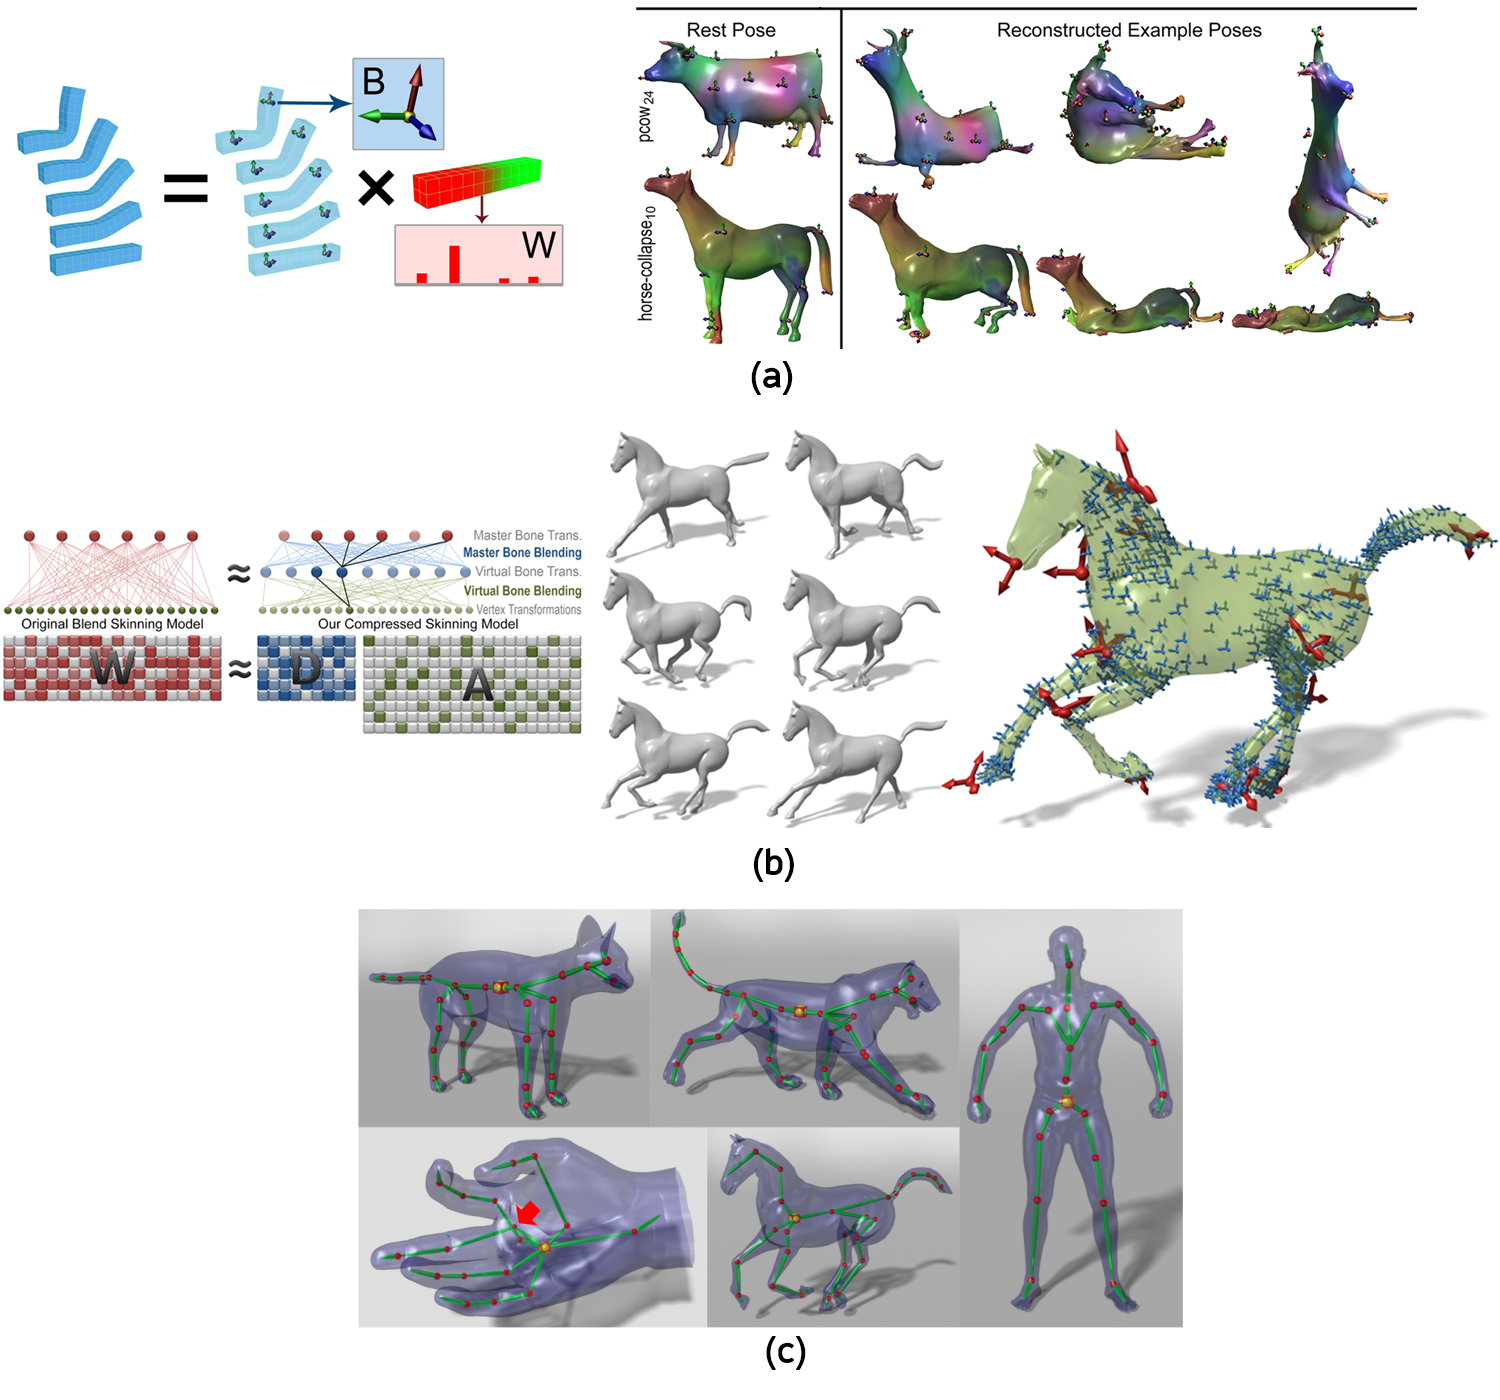
\includegraphics[width=3in]{images/skinning_decomposition}
  \caption{Sparse decomposition: skinning results. (a): \cite{le2012smooth}, left: a set of example poses are decomposed into rigid bone transformation B and a sparse, convex bone-vertex weight map W. right: results of SSDR on elastic models. (b): \cite{le2013two}, left: two-layer scheme. right: an animated mesh sequence and its corresponding compressed skinning model. (c): \cite{le2014ras}.}
\end{figure}


\paragraph{Deformation}

Time-varying dynamic geometry with very fine dynamic shape detail can be generated and rendered at very high visual fidelity. When creating such content, artists usually rely on a low-dimensional control parameterization. Despite increasing expensive power of such parameterizations and simulations, producing such realistic animations from scratch is a labor-intensive process. Following the framework of  sparse PCA\cite{zou2006sparse,jenatton2011structured}, in order to decompose captured or animated mesh sequences into sparse, localized, and intuitive-to-control deformation component, \cite{neumann2013sparse} which propose a method that extracts sparse and spatially localized deformation modes from an animated mesh sequence by extending the theory of sparse matrix decompositions to 3D mesh sequence processing using $l_{1,1}$ norm as the sparse constraint(Figure...).

\begin{figure}[ht]
  \centering
  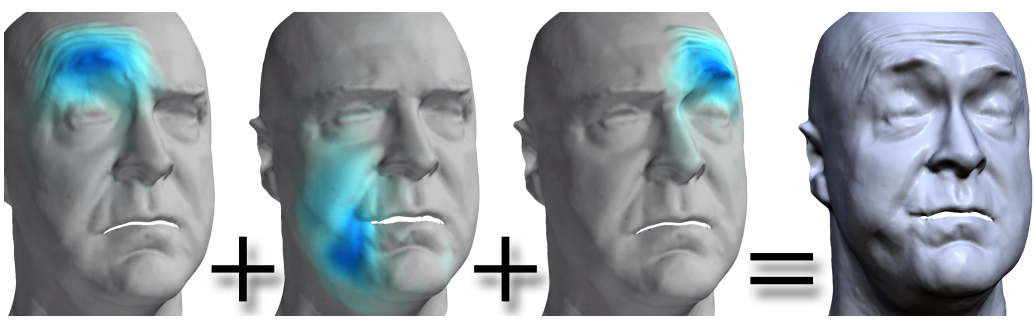
\includegraphics[width=3in]{images/localdefor_learning}
  \caption{Sparse decomposition: deformation\cite{neumann2013sparse}. A new facial expression is generated by summing deformation components.}
\end{figure}


Until now, we haven't given any discussion about the overcomplete dictionary $\mathbf{D}$ that exactly leads to the sparse representations of signals. From the definition of sparse representation, it is obvious that the choice of the dictionary will directly affect the signal processing result. In general, this dictionary can either be chosen as a prespecified set of functions(e.g., wavelet dictionary) or designed by adapting its content to fit a given set of signal examples(e.g., \cite{aharon2006svd}) which is preferred in most signal processing works. Here, we regard it as the sparse decomposition since the representation of a signal is the multiplication of a overcomplete dictionary, which is different from the former simple matrix, and its $sparse$ coefficient. Now that the dictionary could be learned from signals themselves, it could of course simply some processing objects such as point cloud to reduce the computational and memory cost. Compression is no doubt a good application.

\paragraph{Compression}

The compression of unorganized point clouds have also attracted much attention due to the drastic improvement in scanner acquisition devices yielding point sets of tens of millions of points at high precision. But the counterpart of this development are datasets requiring ever higher storage capacity which results in the expensive cost in point cloud processing. \cite{digne2014self} uses the K-SVD algorithm \cite{aharon2006svd}, which seeks the adapting overcomplete dictionaries to achieve the best representation for each element in a training signal set, to encode the local descriptions of the selected seed points which are called self-similarity exploitation. This compression is done at the resolution of the scanner enabling improved control of the point cloud resolution and the input point clouds can be oriented or non-oriented. In addition, the approach also achieves a filtering of noise whose magnitude is smaller that the scanner precision. Figure...shows the compression result.

\begin{figure}[ht]
  \centering
  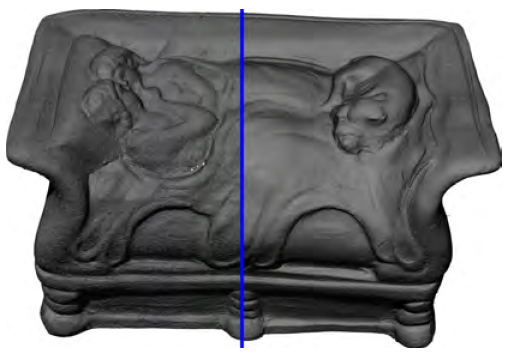
\includegraphics[width=3in]{images/compression_learning}
  \caption{Sparse decomposition: point cloud compression\cite{digne2014self}. The Lovers of Bordeaux(15.8 million points). Exploiting self-similarity in the model, they compress this representation down to 1.15 MB. The resulting model(right) is very close to the original one(left), as the reconstruction error is less than the laser scanner precision(0.02mm) for 99.14\% of the input points.}
\end{figure}

Last year, \cite{miandji2013learning} presents an algorithm for compression and real-time rendering of surface light fields(SLF) encoding the visual appearance of objects in static scenes with high frequency variations. After analyzing the spatial correlation in the data, they use a leaning based approach, Clustered Exemplar Orthogonal Bases(CEOB), to train a compact dictionary of orthogonal basis pairs, enabling efficient sparse projection of the SLF data. This method has an overall advantage in terms of memory footprint, rendering performance and reconstruction error.

\begin{figure}[ht]
  \centering
  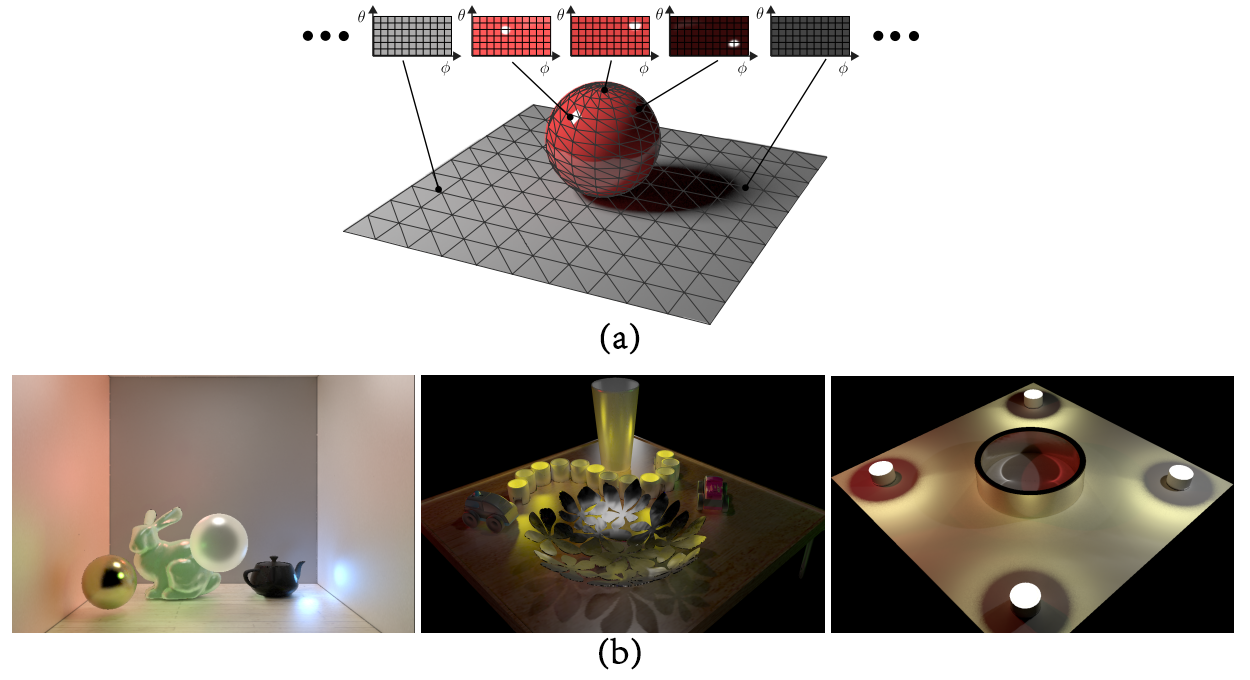
\includegraphics[width=3in]{images/rendering_learning}
  \caption{Sparse decomposition: rendering\cite{miandji2013learning} results using CEOB for three scenes with different materials.}
\end{figure}

\begin{figure}[ht]
  \centering
  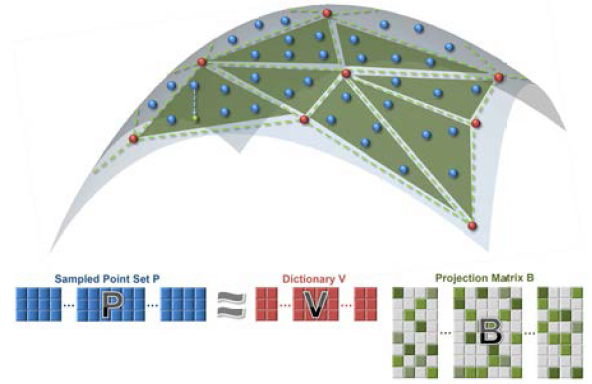
\includegraphics[width=3in]{images/reconstruction_learning}
  \caption{Sparse decomposition: reconstruction\cite{}. Left: an illustration of the reconstruction problem. Right: reconstruction of the Merlion model.}
\end{figure}

\section{Low Rank}
\label{sec:LowRank}


\subsection{Upright orientation}
\label{subsec:upright orientation}

Most man-made models can be posed at a unique upright orientation which is consistent to human sense. Given a 3D digital model, finding its upright orientation and posing it at the right orientation is vital for users to recognize it. However, since produced by various techniques, digital man-made models, such as polygon meshes, might be sloped far from the upright orientation. So how to find the upright orientation would be an useful work.

\begin{figure*}[ht]
  \centering
  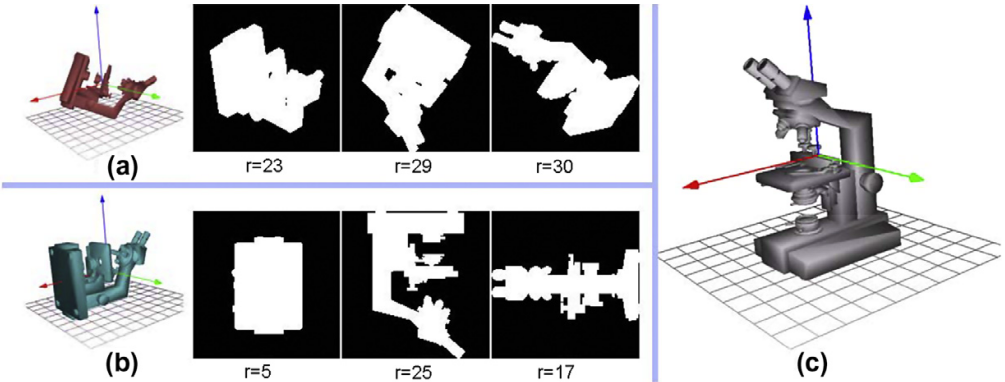
\includegraphics[width=6in]{images/lowrank}
  \caption{Low rank: observation. (a): local method\cite{jin2012unsupervised}. (b): global method\cite{wang2014upright}.}
\end{figure*}

Figure..shows the axis-aligned projections of an input man-made model with arbitrary(a) and axis-aligned orientation(b) onto the $y$-$z$, $y$-$z$ and $y$-$z$ plane(left to right) in the $x$-$y$-$z$(red-green-blue) coordinate system. Regarding these projections as two-domensional matrices, it is clear that the ranks of projection matrices in (b) are significantly $lower$ than those in (a). And, the upright orientation(c) should be one of the six orientations determined by the six axis-aligned candidate bases, i.e., top, bottom, left, right, front and back surface of the bounding box of the model. Briefly, ranks of projection matrices at axis-aligned orientations are lower than their counterparts at other orientations, since man-made models are mainly composed by horizonal and vertical edges and shapes.

\paragraph{(1)}Based on this observation, \cite{jin2012unsupervised} presents an unsupervised approach for finding the upright orientation of man-made models. Taking the $x$-$y$ plane projection as an example, they binarize the projection as black and white to generate the projection image $I$ with fixed resolution which can also be referred as a two-dimensional matrix. And to avoid affect of noise, $I$ can be modeled as a low-rank version $L$ with sparse-error matrix $E$: $I=L+E$. Then the problem is formulated as

\small{
\begin{equation}
 \label{eq:UprightJin}
 \min_{L,E,R}\|L\|_{*}+\lambda\|E\|_{1},~s.t.~I\circ R=L+E
\end{equation}
}
\\
where $\|\cdot\|_{*}$ and $\|\cdot\|_1$ are the nuclear norm(sum of all singular values) and the $L_1$ norm, which are closely related to rank of matrix and sparsity of matrix respectively. $R$ is a rigid rotation transformation matrix which is used to rectify $I$ to recover the optimal low-rank representation of $x$-$y$ plane projection from an arbitrary orientation. After selecting which projection should be rectified from $y$-$z$, $y$-$z$ and $y$-$z$, using () the man-made model will be aligned with some axes followed by final upright orientation selection from six orientations as mentioned above. However, whether a model fits for this algorithm depends on if the model contains dominant parts parallel to the supporting base, then it will fail if the model is composed by several equivalently main parts which have their own low-rank observation in different orientations.%This method can achieve great result when the model has perfect symmetries.

\paragraph{(2)}It is very natural to generalize this method in 3D space to construct three-order tensor(multidimensional array) with volume of the 3D model, i.e., the three-order tensor ought to have a $"$low rank$"$ behavior. \cite{wang2014upright} constructs this three-order tensor using the bounding box of the 3D model since the bounding box parallels the coordinate planes and contains the whole model. By translating the barycenter of the input model to the origin of the coordinate system, they just need to find and optimal rotation matrix $R$ to align the model with three axes by following optimization model

\small{
\begin{equation}
 \label{eq:UprightJin}
 R_{*}=\mathop{\argmin}_{R}(\|\chi(V\circ R)\|_{*})
\end{equation}
}
\\
where $V$ and $V\circ R$ respectively indicate the point coordinates of input model and the rotated model, $\chi(\cdot)$ is the three-order tensor. Similar to \cite{jin2012unsupervised}, after aligning the model with three axes, they select the upright orientation from six orientations by analyzing the geometric properties.
%
%But when a model has not any external symmetry or the symmetry in a big part whose rank plays the leading role in the low-rank optimization is in consistent with the model, the method may fail as well as \cite{jin2012unsupervised}.

\begin{figure}[ht]
  \centering
  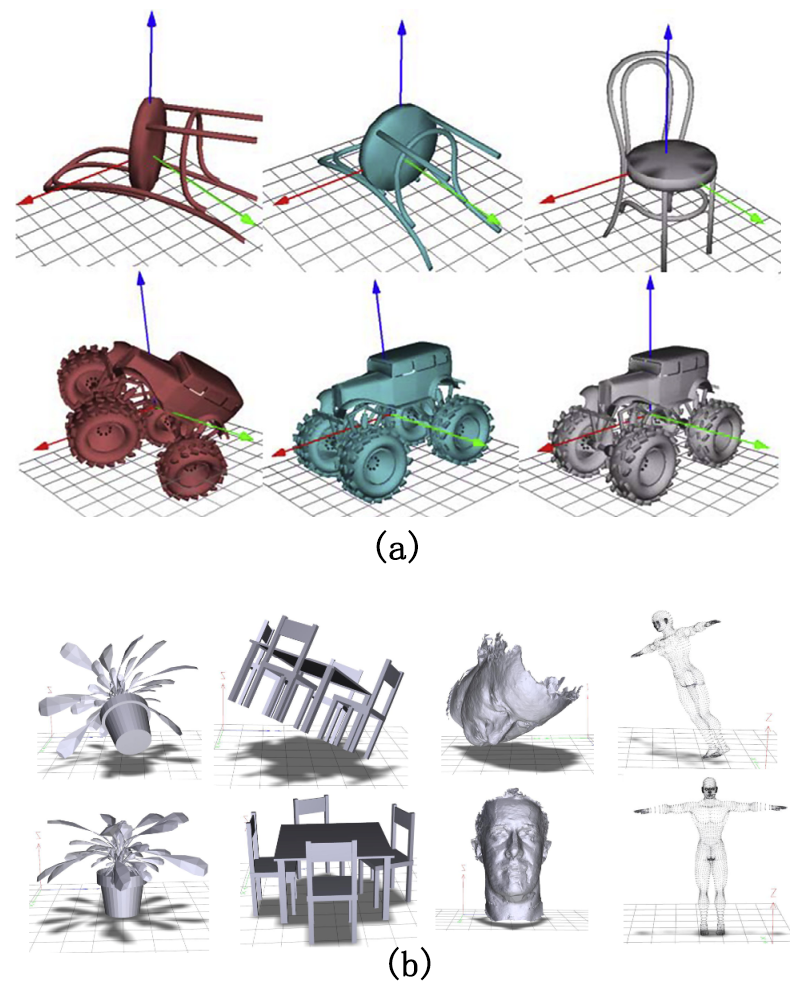
\includegraphics[width=3in]{images/upright_lowrank}
  \caption{Low rank: unsupervised upright orientation. (a): local method\cite{jin2012unsupervised}. (b): global method\cite{wang2014upright}.}
\end{figure} 


\section{Conclusion}
\label{sec:Conclusion} 
\section{Acknowledgements}
\label{sec:Acknowledgements} 

\bibliography{sparsesurvey}

\end{document} 